% !TEX root = ../../../main.tex
% 来源：中学数学实验教材·第三册（高中数学）
% 章节：函数及其图象 / 函数及其图象
% 原始文件：4.tex，行 873-885
% 类型：tikz
% ---
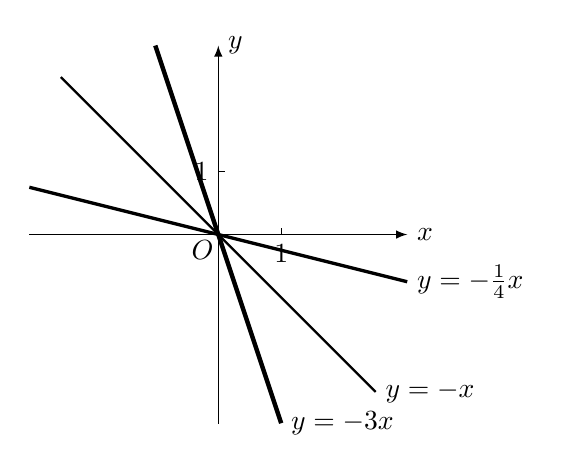
\begin{tikzpicture}[>=latex, scale=.8]
    \draw[->](-3,0)--(3,0)node[right]{$x$};
    \draw[->] (0,-3)--(0,3)node[right]{$y$};
    \node at (-.25,-.25){$O$};
    \draw (1,0)node[below]{1}--(1,.1);
    \draw (0,1)node[left]{1}--(.1,1);
    \draw [thick, domain=-2.5:2.5, samples=100] plot(\x, {-\x});
    \draw [very thick, domain=-3:3, samples=100] plot(\x, {-0.25*\x});
    \draw [ultra thick, domain=-1:1, samples=100] plot(\x, {-3*\x});
    \node at (3,-.75) [right]{$y=-\frac{1}{4}x$};
    \node at (2.5,-2.5) [right]{$y=-x$};
    \node at (1,-3) [right]{$y=-3x$};
\end{tikzpicture}
